
\subsection{New Functionality}
\label{sec:newfunc}

Because {\tt NV\_path\_rendering} is integrated into the OpenGL pipeline
and the coverage information is accessible through the stencil buffer,
we are able to implement unconventional algorithms such as mixing path
rendering with arbitrary 3D graphics.

\begin{figure}[bt]
  \center{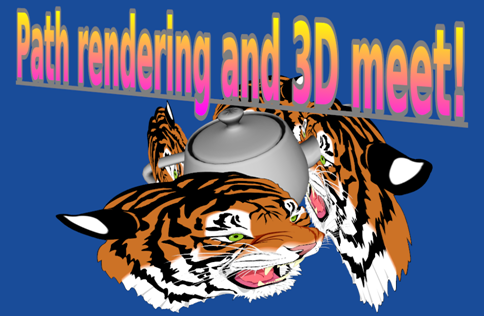
\includegraphics[width=\columnwidth]{tiger3d.png}}
  \caption{\label{fig:tiger3d} Mixing 3D and path rendering in a single
  window.}
\end{figure}

Figure \ref{fig:tiger3d} demonstrates an example of this capability.
No textures are used in this scene.  Arbitrary zooming into the tigers'
detail is supported.  Notice how the tigers properly occlude each other
and the teapot.  Due to the perspective 3D view, the path rendering is
properly rendered in perspective as well.
 
